\documentclass[journal]{IEEEtran}
\usepackage[utf8]{inputenc}
\usepackage{hyperref}
\usepackage[backend=biber]{biblatex}
\usepackage{graphicx}

\addbibresource{main.bib}
\graphicspath{{images/}}

\begin{document}
\markboth{\href{https://github.com/kevinniland97/Literature-review-on-Data-Encryption-algorithms}{Literature review on Data Encryption, its algorithms, and the future of Data Encryption}, December 2019}%
{\href{https://github.com/kevinniland97/Literature-review-on-Data-Encryption-algorithm}{Literature review on Data Encryption, its algorithms, and the future of Data Encryption}, November 2019}

\title{\href{https://github.com/kevinniland97/Literature-review-on-Data-Encryption-algorithms}{Literature review on Data Encryption, its algorithms, and the future of Data Encryption}}
\author{\href{https://github.com/kevinniland97}{Kevin Niland},~\IEEEmembership{Computing in Software Development (Honours),~GMIT}}
\maketitle

\begin{abstract}
Data encryption is integral to many different areas in the computing world. Encryption is used to help protect sensitive data by changing it into a form only readable by a person or entity who has the decryption key. Vast amounts of personal information is managed online and stored in the cloud/servers. With computers becoming increasingly more and more powerful [CHANGE], so too comes the risk that peoples personal information can be accessed by an unauthorized party. As a result, several different algorithms and methods have emerged to prevent this. This paper will look at three different encryption algorithms, the latter two of these algorithms are in use today: the Data Encryption Standard (DES), the Rivest–Shamir–Adleman (RSA) \cite{RSA} and the Advanced Encryption Standard \cite{AES}, which came about 23 years after RSA Encryption and 26 years after DES Encryption. In this paper, both of these algorithms are discussed at length in regards how they came about, their advantages and disadvantages. This paper will also look at the future of data encryption and various methods that could feasibly be proposed as possible replacements for current algorithms and techniques. 
\end{abstract}

\section{\textbf{Introduction}}
Data encryption is a security method where information is encoded and can only be accessed or decrypted by a user with the correct decryption key. Encrypted data, also known as cipher text, appears scrambled or unreadable to a person or entity accessing it without permission. Decrypted data, also known as plain text, appears readable to a person or entity accessing it with permission. Currently, encryption is one of the most popular and effective data security methods used by organizations. A block cipher transforms plain text blocks of a fixed length \textit{${n_b}$} to cipher text blocks of the same length under the influence of a cipher key \textit{k} \cite{block_cipher}. Figure \ref{fig:block_cipher} shows the encryption process.

\newline
\begin{figure}[!hb]
    \centering
    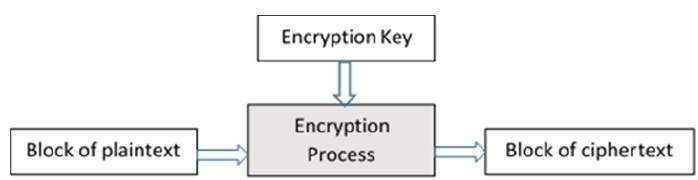
\includegraphics[scale=.3]{block_cipher}
    \caption{Block Cipher}
    \label{fig:block_cipher}
\end{figure}

Two main types of data encryption exist - asymmetric encryption, also known as public-key encryption, and symmetric encryption. Asymmetric encryption came about after symmetric encryption, as an answer for secure communications with an emphasis on applications that could not have been satisfactorily handled by cryptographic techniques at the time \cite{asymm_symm}. % While there are several types of encryption methods and algorithms, this paper will focus on two specific algorithms: RSA encryption (a form of asymmetric encryption) which was first publicly described in 1977 by Ron Rivest, Adi Shamir, and Leonard Adleman, and AES encryption (a form of symmetric encryption) which was first announced in 2000 by NIST and developed by Vincent Rijmen and Joan Daemen. % Symmetric encryption uses a single password to encrypt and decrypt data. Asymmetric encryption uses two keys for encryption and decryption. A public key, which is shared among users, encrypts the data. A private keencryption, each developed with different needs and security needs in mind, this literaturey, which is not shared, decrypts the data. While there are several types of encryption methods and algorithms, this review will focus on two specific algorithms: RSA encryption (a form of asymmetric encryption) which was first publicly described in 1977 by Ron Rivest, Adi Shamir, and Leonard Adleman, and AES encryption (a form of symmetric encryption) which was first announced in 2000 by NIST and developed by Vincent Rijmen and Joan Daemen. %Additionally, this paper will also focus on future encryption systems and possible replacements of existing encryption algorithms, including but not limited to RSA encryption and AES encryption.

\subsection{\textbf{History of Data Encryption}}
Data encryption, in one form or another, has existed for almost 3000 years. Circa 600 B.C., Spartans used a device called a scytale to send secret messages during a battle. Circa 60 B.C., Julius Caesar invented a substitution cipher that shifted characters by three places. A becomes D, B becomes E, and so on. In 1553, Giovan Battista Bellaso envisioned the first cipher to use a proper encryption key - an agreed-upon keyword that the recipient needs to know if he or she wants to decode the message. In 1795, Thomas Jefferson invented Jefferson's Wheel Cipher which was later used in the United States Army from 1923 to 1942. However, interestingly, the army never knew about Jefferson's invention. They simply re-invented it and called it the 'M-64'. In 1854, Charles Wheatstone invented the Playfair Cipher, which encrypted pairs of letters instead of single ones and was therefore harder to crack.

\subsection{\textbf{Current Status of Data Encryption}}
Over time, however, the above mentioned methods have been proved to be insecure since an eavesdropper - known as cryptanalysts - could exploit simple statistical features of the cipher text to easily recover the plain text and even the decryption key, allowing them to easily decypher any future messages using that system \cite{encryption_today}. Modern computing technology has made it practical to use far more complex encryption algorithms that are harder to “break” by cryptanalysts. In parallel, cryptanalysts have adopted and developed this technology to improve their ability to break cryptosystems \cite{des_cryptanalysis}, \cite{rijndael_cryptanalysis}, \cite{rsa_cryptanalysis}. 

\section{\textbf{Symmetric Encryption}}
Symmetric encryption is a form of data encryption where the encryption key and the corresponding decryption key are the same. The persons or entities communicating via symmetric encryption must exchange the key so that it can be used in the decryption process. This encryption method differs from asymmetric encryption where a pair of keys, one public and one private, is used to encrypt and decrypt messages. To discuss symmetric encryption, this paper will look at the first standardized cipher which was the Data Encryption System (DES). 
\newline \newline
The Data Encryption Standard (DES) was first published in 1975, standardized in 1977 and ultimately withdrawn as the standard by the National Institute of Standards and Technology in 2001 \cite{DES}. It was the first publicly available cryptographic algorithm that was endorsed by the U.S. government. Figure \ref{fig:des} shows the DES structure.
\newline
\newline
\begin{figure}[!h]
    \centering
    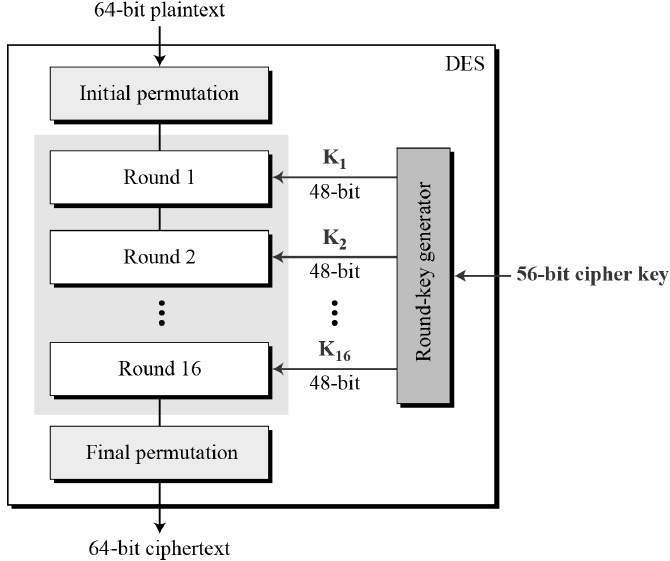
\includegraphics[scale=.3]{des_structure}
    \caption{DES Structure}
    \label{fig:des}
\end{figure}

During this time the standard was revised three times: as FIPS-46-1 in 1988, as FIPS-46-2 in 1993 and as FIPS-46-3 in 1999. DES was an outcome of a call for primitives in 1974, which did not result in many serious candidates except for a predecessor of DES, Lucifer, designed by IBM around 1971 \cite{DES}. As discussed in Miles E. Smid and Dennis K. Branstad's paper, \textit{"The Data Encryption Standard: Past and Future"}, the DES security controversy \cite{DES_past&future} forced security questions about how good is good enough and how long is long enough. This controversy came about due to DES short key length of 56 bits, which was criticized from the beginning. Although this made it too insecure for most current applications (this is evidenced by the fact that it was cracked in 1997 \cite{des_cracked}), it was highly influential in the advancement of modern cryptography \cite{des_overview} and in the year 2000, it was replaced by the Advanced Encryption Standard (AES) which was found through a competition open to the public.
\newline\newline
The Advanced Data Encryption Standard (AES), originally known as Rijndael, was developed by Vincent Rijmen and Joan Daemen. AES is a subset of the Rijndael block cipher. It was first announced in 2000 by NIST as the surprise winner \cite{AES} of its Advanced Data Encryption Standard competition. It subsequently replaced DES in 2001 \cite{Encryption_Study}. Figure \ref{fig:aes} shows the AES structure.

\newline
\begin{figure}[!h]
    \centering
    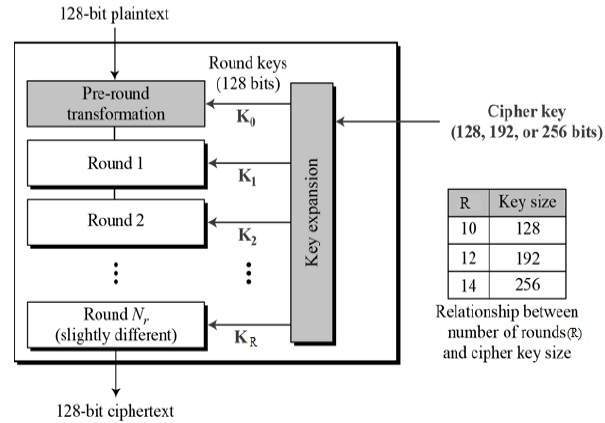
\includegraphics[scale=.267]{aes_structure}
    \caption{AES Structure}
    \label{fig:aes}
\end{figure}

Rijndael is a family of ciphers with different key and block sizes. AES and Rijndael differ only in terms of the range of supported values for the block length and cipher key length. In terms of the block length, Rijndael has a minimum of 128 bits and a maximum of 256 bits. AES has a fixed block length of 128 bits. In terms of the key length, Rijndael supports any length that is a multiple of 32 bits. AES supports key lengths of 128, 192, or 256 only \cite{aes_rijndael_length}. Since its inception, it has been adopted by the U.S. government and is now also used worldwide. AES is based on a design principle, known as substitution–permutation network. A substitution–permutation network is a series of linked mathematical operations used in block cipher algorithms \cite{sp_network}. Unlike DES, AES doesn't use a Feistel network/cipher, which is symmetric structure used in the construction of block ciphers.... One problem with AES Encryption is that it has slow computation. As described in Rizky Riyaldhi, Rojali, and Aditya Kurniawan's paper, \textit{"Improvement of Advanced Encryption Standard Algorithm With Shift Row and S.Box Modification Mapping in Mix Column"}, their experiments showed that it takes 3.045 milliseconds to compute 1024 bytes of data. This increases by 3 - 4 milliseconds for 2048 bytes of data and so on \cite{aes_improvement}. Figure \ref{fig:aes_times} shows the computational times published in Rizky Riyaldhi, Rojali, and Aditya Kurniawan's paper.

\newline
\begin{figure}[!h]
    \centering
    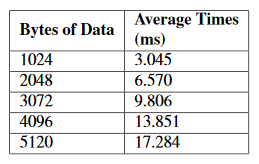
\includegraphics[scale=.7]{aes_times}
    \caption{AES Computational Times}
    \label{fig:aes_times}
\end{figure}

In the same paper, however, they proposed a method to improve the AES algorithm through the use of Shift Row and S. Box modification for Mix Column transformation. Shift Row is a circular process that shifts bytes in each row of a matrix by a certain offset, which is determined by the encryption algorithm \cite{shift_row}. For Rizky Riyaldhi, Rojali, and Aditya Kurniawan's paper, the shift row process started from the 2nd row to the 4th row. 

\newline
\begin{figure}[!h]
    \centering
    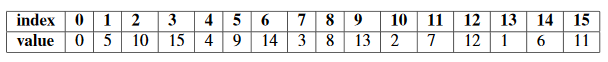
\includegraphics[scale=.5]{shift_row}
    \caption{Shift Row}
    \label{fig:aes_times}
\end{figure}

The result of this showed that the computational time of AES was reduced by 3 milliseconds. 

\newline
\begin{figure}[!h]
    \centering
    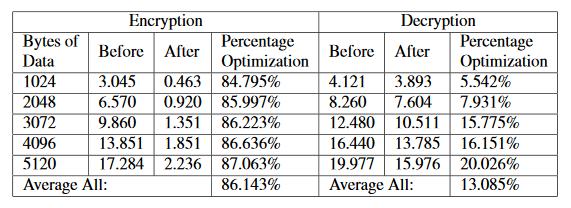
\includegraphics[scale=.7]{aes_improvement}
    \caption{AES Improvement}
    \label{fig:aes_times}
\end{figure}

\section{\textbf{Asymmetric Encryption}}
Asymmetric encryption, also known as public-key encryption, is a form of data encryption where the encryption key (also called the public key) and the corresponding decryption key (also called the private key) are different. This paper will look at a specific asymmetric encryption algorithm, the Rivest–Shamir–Adleman algorithm. The Rivest-Shamir-Adleman (RSA) algorithm, was designed by Ron Rivest, Adi Shamir, and Leonard Adleman in 1978. The asymmetry of RSA is based on the practical difficulty of the factorization of the product of two large prime numbers, named "prime factorisation" \cite{prime_factorization}. Based on number theory, which is a block cipher system, it is one of the most widely known public key cryptosystems. It is used for key exchange, digital signatures, or encryption of blocks of data. RSA uses a variable size encryption block and a variable size key. The most notable advantage of the RSA algorithm is that since it's a public-key cipher, it makes it easier to to solve the fundamental problem of cryptography - how to safely distribute keys. Public crytography solved this dilemma by having two different keys - one key for encryption and one key for decryption. To generate the public keys (for encryption) and private keys (for decryption), it uses two prime numbers. The basic operation of the RSA algorithm goes as follows: Figure \ref{fig:rsa} shows the operation of the Rivest-Shamir-Adleman (RSA) algorithm:

\newline
\begin{figure}[!h]
    \centering
    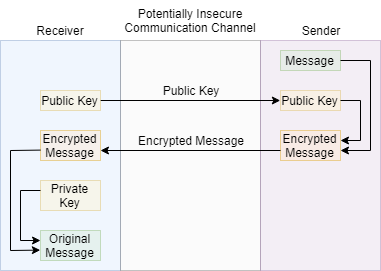
\includegraphics[scale=.5]{rsa}
    \caption{RSA Process}
    \label{fig:rsa}
\end{figure}

The Sender encrypts the message using the Receiver's public key. Once the message has been successfully transmitted to the Receiver, the Receiver can then decrypt the message using their own private key. When RSA was introduced, it implemented two important principles: public-key encryption and digital signatures \cite{RSA}. The RSA operation(s) can be broken down into three broad steps: key generation, encryption, and decryption. While RSA has its advantages, it has many flaws and is subsequently not suitable or preferred for commercial use. As discussed in Gurpreet Singh and Supriya's article, "\textit{A Study of Encryption Algorithms (RSA, DES, 3DES and AES) for Information Security}", if two values \textit{p} and \textit{q} (where \textit{p} and \textit{q} are distinct prime numbers such that \textit{p} $\neq$ \textit{q}) are too small when designing the key, then the encryption process becomes too weak and one would be able to decrypt the data by using random probability theory and side channel attacks. Conversely, if \textit{p} and \textit{q} are too big when designing the key, the encryption process consumes more time and the performance gets degraded in comparison to DES \cite{Encryption_Study}. 

\section{\textbf{Future of Data Encryption and Possible Replacements of Existing Encryption Algorithms}}
There are several different techniques that could possibly be employed in the future to further enhance our ability to encrypt and decrypt our data. Some of these have been and still are being extensively researched and tested. Some examples include, but are not limited to: Elliptic Curve Cryptography (ECC) \cite{ecc}, Quantum Computation \cite{quantum_computing_encryption}, and a new data encryption algorithm based on the location of mobile users which has been given the name, "Location-Dependent Data Encryption Algorithm (LDEA)" \cite{new_encryption_mobile} has also been proposed.

\subsection{\textbf{Elliptic Curve Cryptography (ECC)}}
Elliptic-curve cryptography (ECC) is an approach to public-key cryptography based on the algebraic structure of elliptic curves over finite fields. In Nicholas G. McDonald's research review, "Past, Present, and Future Methods of Cryptography and Data Encryption" \cite{encryption_research}, he discussed in brief Elliptic Curve Cryptography. As he stated, he states that Elliptic Curve Cryptography has technically already been invented but he considered it to be a future technique of cryptography because its advantages and disadvantages are not yet fully understood. In terms of encryption, ECC is an approach that utilizes the complex nature of elliptic curves in finite fields. A finite field (also called a Galois field, so named in honor of Évariste Galois, a French mathematician) in mathematics is a field that contains a finite number of elements. While RSA encryption and ECC typically use the same types of algorithms, the difference is that the numbers used are chosen from a finite field defined within an elliptic curve expression.

\newline
\begin{figure}[!h]
    \centering
    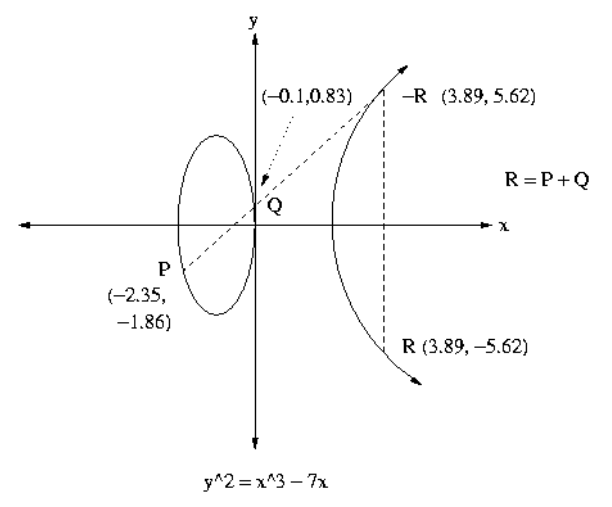
\includegraphics[scale=.5]{elliptic_curve}
    \caption{Elliptic Curve Cryptography}
    \label{fig:ecc}
\end{figure}

\subsection{\textbf{Quantum Cryptography}}
Integer factorization, which underpins the security of public key cryptographic systems, is believed to be computationally infeasible with an ordinary computer for large integers if they are the product of few prime numbers (e.g., products of two 300-digit primes). Nicholas G. McDonald's also briefly discussed the possibility of using Quantum Computation as future method of data encryption in his research review \cite{encryption_research}. Quantum Computation is performed in a quantum computer or processor, which is a processor that makes use of quantum mechanical phenomena, such as quantum superposition and quantum entanglement. Quantum superposition is a fundamental principle of quantum mechanics. Much like waves in classical physics, it states that any two (or more) quantum states can be added together - superimposes - and the result will be another valid quantum state. Using quantum logical qubit state, which is quantum superposition of the "basis states" 0 and 1 as an example, a superposition is where a qubit can be in the state 0 and 1 at the same time, contrary to a classical bit which can only be in the state corresponding to state 0 or the state corresponding to 1. Depending on the quantum design, each qubit can store a set number values simultaneously. Quantum computing is still in its infancy and, as a result, quantum processors manufactured today are very small and do not have the computational size that transistor processors have. Some fear that a successful and practical quantum computer would devastate the world's financial system by breaking every encryption system known - public-key cryptography relies on computer being slow to compute discrete logarithms and prime factorizations. Figure \ref{fig:rot} shows a new quantum-cryptography scheme, Random Oblivious Transfer (ROT), to secure anonymous transactions.

\newline
\begin{figure}[!h]
    \centering
    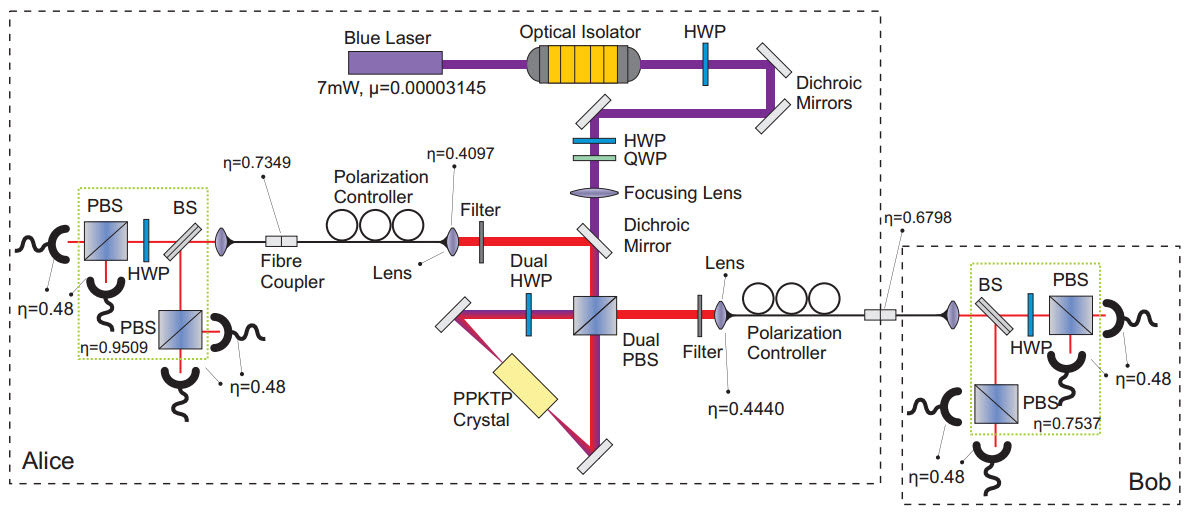
\includegraphics[scale=.3]{ROT-experiment}
    \caption{Random Oblivious Transfer (ROT)}
    \label{fig:rot}
\end{figure}

\subsection{\textbf{Location-Dependent Data Encryption Algorithm (LDEA)}}
As proposed in Hsien-Chou Liao and Yun-Hsiang Chao's 2008 study, "A New Data Encryption Algorithm Based on the Location of Mobile
Users" \cite{new_encryption_mobile}, most of the data encryption technology is location-independent. That is, encrypted data can be decrypted anywhere. Encryption technology of today is unable to restrict the location of the decryption of data. Hsien-Chou Liao and Yun-Hsiang Chao proposed the idea of a location-dependent approach, named Location-Dependent Data Encryption Algorithm (LDEA). 

\newline
\begin{figure}[!h]
    \centering
    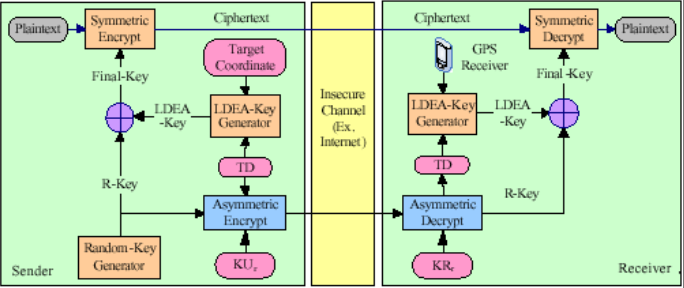
\includegraphics[scale=.6]{ldea}
    \caption{Location-Dependent Data Encryption Algorithm (LDEA)}
    \label{fig:ldea}
\end{figure}

For this approach to work, a target latitude and longitude coordinate is determined firstly. The coordinate is then incorporated with a random key for data encryption. As a result, the receiver can only decrypt the cipher text when the coordinate acquired from the GPS receiver is matched with the target coordinate. A number of drawbacks to modern technology, such as GPS that would be used in this approach, renders LDEA difficult to implement well. The location of a mobile user is difficult to exactly match with the target coordinate due to current GPS receivers being inaccurate and inconsistent.
\newline\newline
In Hatem Hamad and Souhir Elkourd's research paper, "Data encryption using the dynamic location and speed of mobile node", they proposed a simialar idea to that of the one proposed by Hsien-Chou Liao and Yun-Hsiang Chao in their paper. They proposed a method of key security where the receiver MN (Mobile Node) registers some coordinates and speed during the travel and thus can chart the course of movement \cite{encryption_mobile_node}. Through this path, one can predict the next coordinate expected after a certain amount of time since the GPS receiver is inaccurate and inconsistent, depending on how many satellite signals are received, as mentioned in Hsien-Chou Liao and Yun-Hsiang Chao's paper. However, as stated in Hatem Hamad and Souhir Elkourd's research paper, Hsien-Chou Liao and Yun-Hsiang Chao's protocol isn't strong enough due to them using the static location  (the longitude and latitude coordinates of the mobile node). To overcome the inaccuracy and inconsistency of a GPS receiver, they also use a static Tolerance Distance (TD). In contrast, Hatem Hamad and Souhir Elkourd applied a dynamic location of the mobile node and TD which greatly improves the security of the protocol \cite{encryption_mobile_node}.

\section{\textbf{Conclusion}}
This paper reviewed data encryption in regards to  main areas: the history of data encryption, the current state of data encryption, where this paper looked at two specific forms of data encryption algorithms - the Rivest–Shamir–Adleman algorithm (RSA), the Data Encryption Standard (DES) and its successor the Advanced Data Encryption Standard (AES). From this, it is clear that data encryption is a highly important aspect for today's technology and is widely researched in the area of Computer Science. Along with this, it is also evident from this paper that the field of data encryption will continue to progress and grow exponentially with new methods of data encryption, such as Elliptic Curve Cryptography and Location-Dependent Data Encryption Algorithm (LDEA), being continually researched and tested. As Quantum Computing continues to grow in popularity and accessibility, this also opens up the possibility of different avenues of data encryption being explored and potentially implemented in the coming years.

\bigskip

\printbibliography[title={References}]
\cite{DES}
\cite{DES_past&future}
\cite{des_cryptanalysis}
\cite{des_overview}
\cite{des_cracked}
\cite{AES}
\cite{aes_improvement}
\cite{rijndael_cryptanalysis}
\cite{aes_rijndael_length}
\cite{RSA}
\cite{rsa_cryptanalysis}
\cite{Encryption_Study}
\cite{prime_factorization}
\cite{block_cipher}
\cite{asymm_symm}
\cite{encryption_today}
\cite{sp_network}
\cite{shift_row}
\cite{encryption_research}
\cite{new_encryption_mobile}
\cite{quantum_computing_encryption}
\cite{encryption_mobile_node}
\cite{ecc}
\end{document}
